%
% File acl2020.tex
%
%% Based on the style files for ACL 2020, which were
%% Based on the style files for ACL 2018, NAACL 2018/19, which were
%% Based on the style files for ACL-2015, with some improvements
%%  taken from the NAACL-2016 style
%% Based on the style files for ACL-2014, which were, in turn,
%% based on ACL-2013, ACL-2012, ACL-2011, ACL-2010, ACL-IJCNLP-2009,
%% EACL-2009, IJCNLP-2008...
%% Based on the style files for EACL 2006 by 
%%e.agirre@ehu.es or Sergi.Balari@uab.es
%% and that of ACL 08 by Joakim Nivre and Noah Smith

\documentclass[11pt,a4paper]{article}
\usepackage[hyperref]{acl2020}
\usepackage{times}
\usepackage{latexsym}
\renewcommand{\UrlFont}{\ttfamily\small}
\usepackage{booktabs}
\usepackage{tikz}
\usepackage{amsmath}
\usepackage{graphicx}
\usepackage{natbib}
% This is not strictly necessary, and may be commented out,
% but it will improve the layout of the manuscript,
% and will typically save some space.
\usepackage{microtype}

%\aclfinalcopy % Uncomment this line for the final submission
%\def\aclpaperid{***} %  Enter the acl Paper ID here

%\setlength\titlebox{5cm}
% You can expand the titlebox if you need extra space
% to show all the authors. Please do not make the titlebox
% smaller than 5cm (the original size); we will check this
% in the camera-ready version and ask you to change it back.

\newcommand\BibTeX{B\textsc{ib}\TeX}

\title{Instructions for ACL 2020 Proceedings}

\author{First Author \\
  Affiliation / Address line 1 \\
  Affiliation / Address line 2 \\
  Affiliation / Address line 3 \\
  \texttt{email@domain} \\\And
  Second Author \\
  Affiliation / Address line 1 \\
  Affiliation / Address line 2 \\
  Affiliation / Address line 3 \\
  \texttt{email@domain} \\}

\date{}

\begin{document}
\maketitle
\begin{abstract}
  Basically we want to see if language models pre-trained on text data are useful for dialogue.
  So we look at if BERT is useful for dialouge act recoginiton.
  But we want to know if it's really adapting to the domain, so we look at how it uses laughter, a phenomenon specific to dialogue.
\end{abstract}

% INTRODUCTION

Recently, large-scale language models, trained on massive corpora of text data, have achieved state-of-the-art results on a variety of traditonal NLP tasks.
We investigate whether such models might be useful for processing dialogue, and if so, whether they adapt to make use of dialogue-specific features.

Dialogue, especially spoken dialogue, is radically different from the kind of data that neural language models are prestrained on.
Not only is the internal structure of contributions different---with features such as disfluencies, repair, incomplete sentences, and various vocal sounds---but the sequential structure of the discourse is also very different.
In dialouge speakers take turns and switch perpsectives.
More generally, the way that utterances contribute and cohere to the discourse is different from the relationship between sentences in a piece of written text.

One important dialogical feature missing from text data is laughter.
In the Switchboard dialogue corpus, laughter appears in approximately \%X of utterances.
Laughter also relates to the discourse structure of dialogue. 
% Laughables.
Also useful for predicting DAs (is that already a result?)

In this work, we investigate whether BERT, a well-know pre-trained language model, is useful for dialogue.
We use dialogue act recoginition as a proxy task, since both the interal content of conributions, and their sequential structure have bearing on the task.

\paragraph{Contributions}
The main results of this paper have to do with to the usefulness of language model fine-tuning for DAR, 
the impact of laughter on DAR, and the relationship between the two.
\begin{itemize}
  \item Laughter is useful for dialogue act recoginition (\S\ref{sec:experiment1}).
  \item The impact of laughter is different for different dialogue acts. [Bigger for forward/backward?] (\S\ref{sec:experiment1})
  \item Standard BERT pre-traininig is useful for DAR, but the impact of pre-training is smaller than than of fine-tuning (\S\ref{sec:experiment2})
  \item 
\end{itemize}


\section{Background} % Vlad
%  - dialogue acts
%  - laughter
%  - BERT 

References
\begin{itemize}
  \item \citet{austinHowThingsWords2009} -- speeh acts
  \item \citet{coreCodingDialogsDAMSL1997} -- DAMSL dialogue act tagging scheme. SWDA tags are based on this (I think AMI are too). Concept of multi-layer DA tags; forward/backward function
  \item \citet{jurafskySwitchboardSWBDDAMSLShallowDiscourseFunction1997a} -- SWBD-DAMSL coders manual
  \item \citet{devlinBERTPretrainingDeep2018} -- Original BERT paper
  \item \citet{sunHowFineTuneBERT2019} -- recommendations for fine-tuninig BERT
  \item \citet{mikolovDistributedRepresentationsWords2013} -- word2vec
  \item \citet{petersTuneNotTune2019} -- when and how to fine-tune pre-trained representations
  \item \citet{kimConvolutionalNeuralNetworks2014} -- CNN sentence representation
  \item \citet{stolckeDialogueActModeling2000} -- OG DAR model. Uses an HMM with various lexical and prosodic features
\end{itemize}

\section{Data}
We perform experiments on the Switchboard Dialogue Act Corpus (SWDA), which is a subset of the larger Switchboard corpus, and the dialogue act-tagged portion of the AMI Meeting Corpus (AMI-DA).

% - DA distribution              % Vlad
% - Laughter frequencies per DA  % Vlad

% - AMI, SWBD + comparison table % Bill
\begin{table}[]
\centering
\begin{tabular}{@{}ll@{}}
\toprule
\textbf{Switchboard}       & \textbf{AMI Corpus}                     \\ \midrule
Dyadic                     & Multi-party                             \\
Casual conversation        & Mock business meeting                   \\
Telephone                  & In-person \& video                      \\ \midrule
English                    & English                                 \\ 
Native speakers            & Native \& non-native speakers           \\ 
early '90s                 & 2000s                                   \\ \midrule
2200 conversations         & 171 meetings                            \\
  \hspace{1em} 1155 in SWDA               & \hspace{1em} 139 in AMI-DA                           \\
400k utterances             & 118k utterances                         \\
3M tokens                  & 1.2M tokens                             \\ \bottomrule
\end{tabular}
  \caption{Comparison between Switchboard and the AMI Meeting Corpus}
  \label{table:corpora}
\end{table}

% - Preprocessing: remove disfluencies, acronyms and speaker tokens in AMI, removing laughter % Bill
  
\section{Model} % Bill

We employ a simple DAR model with two components: an encoder that vectorizes utterances, and a sequence model that predicts dialogue act tags from the vectorized utterances (figure \ref{fig:model-architecture}).
Since we are primarily interested in comparing different utterance encoders, we use a simple RNN as the sequence model in every configuration. 
The RNN takes the encoded utterance as input at each time step
Its hidden state is passed to a simple linear classification layer over dialogue act tags.
Conceptually, the encoded utterance represents the context-agnostic semantic content of the utterance, and the hidden state of the RNN represents the discourse context.

As a baseline utterance encoder, we use a word-level CNN with window sizes of 3, 4, and 5, each with 100 feature maps \citep{kimConvolutionalNeuralNetworks2014}. 
The model uses 100-dimensional word embeddings, which are initialized with pre-trained gloVe vectors in some configurations \citep{penningtonGloveGlobalVectors2014}.

For the BERT utterance encoder, we use the BERT-BASE model with hidden size of 768 and 12 transformer layers and self-attention heads \citep[][see \S3.1]{devlinBERTPretrainingDeep2018}.
We use the un-cased model implemented by \citet{wolfHuggingFaceTransformersStateoftheart2019}.

\begin{figure*}
  
\tikzstyle{rnn}=[rectangle,
  thick,
  minimum height=0.5cm,
  minimum width=2cm,
  fill=cyan]
\tikzstyle{encoder}=[rectangle,
  thick,
  minimum height=0.5cm,
  minimum width=2cm,
  fill=yellow]

\centering
\begin{tikzpicture}[>=latex,text height=1.5ex,text depth=0.25ex]
  \matrix[row sep=0.5cm,column sep=0.5cm] {
  % First line: Output labels
  \node (Y_0) []{$\hat{Y}_0$};&
  \node (Y_1) []{$\hat{Y}_1$};&
  \node (dots1) [] {$\dots$};  &
  \node (Y_T) []{$\hat{Y}_T$};&
  \\ % Second line: RNNs
  \node (RNN_0) [rnn]{RNN};&
  \node (RNN_1) [rnn]{RNN};&
  \node (dots2) [] {$\dots$};  &
  \node (RNN_T) [rnn]{RNN};&
  \\ % Third line: Linear layers
  \node (Encoder_0) [encoder]{Encoder};&
  \node (Encoder_1) [encoder]{Encoder};&
  \node (dots3) [] {$\dots$};  &
  \node (Encoder_T) [encoder]{Encoder};&
  \\ % Fourth line: Linear layers
  \node (Input_0) []{\small $ \underbrace{s^0,w^0_{0},w^0_{1},...,w^0_{n_0}}_{\text{Utterance 1}}$};&
  \node (Input_1) []{\small $ \underbrace{s^1,w^1_{0},w^1_{1},...,w^1_{n_1}}_{\text{Utterance 2}}$};&
  \node (dots4) [] {$\dots$};  &
  \node (Input_T) []{\small $ \underbrace{s^T,w^T_{0},w^T_{1},...,w^T_{n_T}}_{\text{Utterance T}}$};&
  \\ };
  \path[->]
  (Input_0) edge[thick]  (Encoder_0)	
  (Input_1) edge[thick] (Encoder_1)	
  (Input_T) edge[thick] (Encoder_T)	

  (Encoder_0) edge[thick] node[right] {} (RNN_0)	
  (Encoder_1) edge[thick] node[right] {} (RNN_1)	
  (Encoder_T) edge[thick] node[right] {} (RNN_T)	

  (RNN_0) edge[thick] (Y_0)	
  (RNN_1) edge[thick] (Y_1)	
  (RNN_T) edge[thick] (Y_T)	

  (RNN_0) edge[thick] node[above] {$h_1$} (RNN_1)
  (RNN_1) edge[thick] node[above] {$h_2$} (dots2)
  (dots2) edge[thick] node[above] {$h_T$} (RNN_T)
  ;
\end{tikzpicture}

  \caption{DAR model architecture}
  \label{fig:model-architecture}
\end{figure*}
%  - DAR model -> utt encoder, RNN sequence tagger
%  - BERT encoder (12 heads, uncased,...)
%  - baseline encoder

\section{Experiments}
\subsection{Experiment 1: Impact of laughter} \label{sec:experiment1}   % Vlad
In the first experiment we investigated whether laughter, as an example of a dialogue-specific signal, is a helpful feature for DAR.
Therefore, we train another version of each model: one containing laughs (\texttt{L}) and one with laughs left out (\texttt{NL}), and compare their performances in DAR task.
Table~\ref{table:laughter-total-acc}) compares the results from applying the models with two different different utterance encoders (\texttt{BERT}, \texttt{CNN}). From observing the total accuracy scores, models appear to be almost unaffected by leaving out the laughters. On the other hand, we can observe differences in performance depending on the dialogue act, regardless how often laughter occurs in the current or adjacent utterances (see Figure~\ref{fig:swda-by-da} for Switchboard and Figure~\ref{fig:ami-by-da} for AMI corpus).

In order to further investigate the differences we have grouped dialogue acts in Switchboard according to DAMSL coders manual \citep{jurafskySwitchboardSWBDDAMSLShallowDiscourseFunction1997a}. Different DA groups containing 
\begin{table}
  \centering
  \begin{tabular}{@{}lll@{}}
    \toprule
                      & SWDA  & AMI-DA   \\ \midrule
    \texttt{BERT-NL}  & 77.07 & 67.06       \\ 
    \texttt{BERT-L}   & 76.93 & 67.12       \\ \midrule
    \texttt{CNN-NL}   & 75.08 & 63.46        \\
    \texttt{CNN-L}    & 75.40 & 64.30        \\ \bottomrule
    
  \end{tabular}
  \caption{Comparison of models depending on using laughter on the training phase. }
  \label{table:laughter-total-acc}
\end{table}

\begin{table}
  \label{tab:laughter}
  \centering
  \begin{tabular}{@{}lccc@{}}
    \toprule
    & \%lassoc & \%L  & $\Delta$ (mean acc.) \\ \midrule
    Forward-CF & 11.86 & 4.59 & 11.40\\
    Backward-CF & 11.57 & 3.03 & 4.30\\
    Other & 12.71 & 4.40 & 2.39\\
    CS & 20.63 & 14.17 & -1.50\\\bottomrule
    
  \end{tabular}
  \caption{Laughter impact by dialogue act group (SWDA, BERT), mean accuracy}
\end{table}


\begin{figure*}
  \centering
  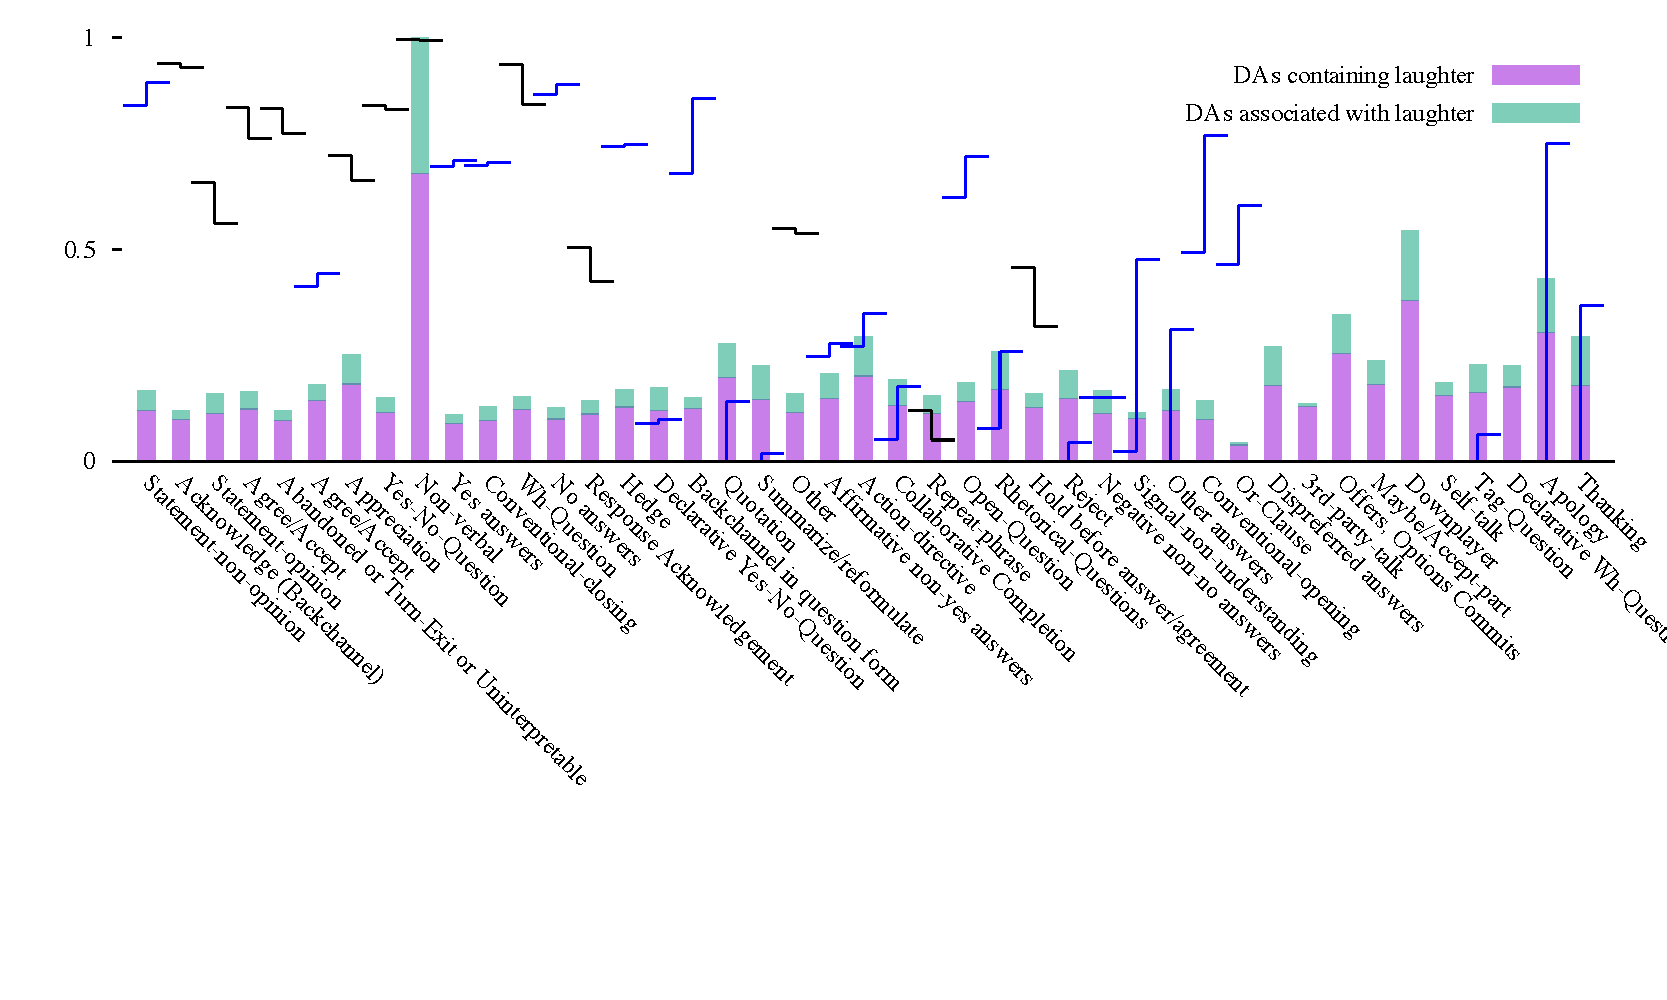
\includegraphics[width=\textwidth]{img/SWDA-bertLvsNL.pdf}
  \caption{Change in accuracy for each SWDA dialogue act. Positive changes when adding laughter are shown in blue. Vertical bars indicate how often dialogue act is associated with laughter.}
    \label{fig:swda-by-da}
\end{figure*}

\begin{figure*}
  \label{fig:ami-by-da}
  \centering
  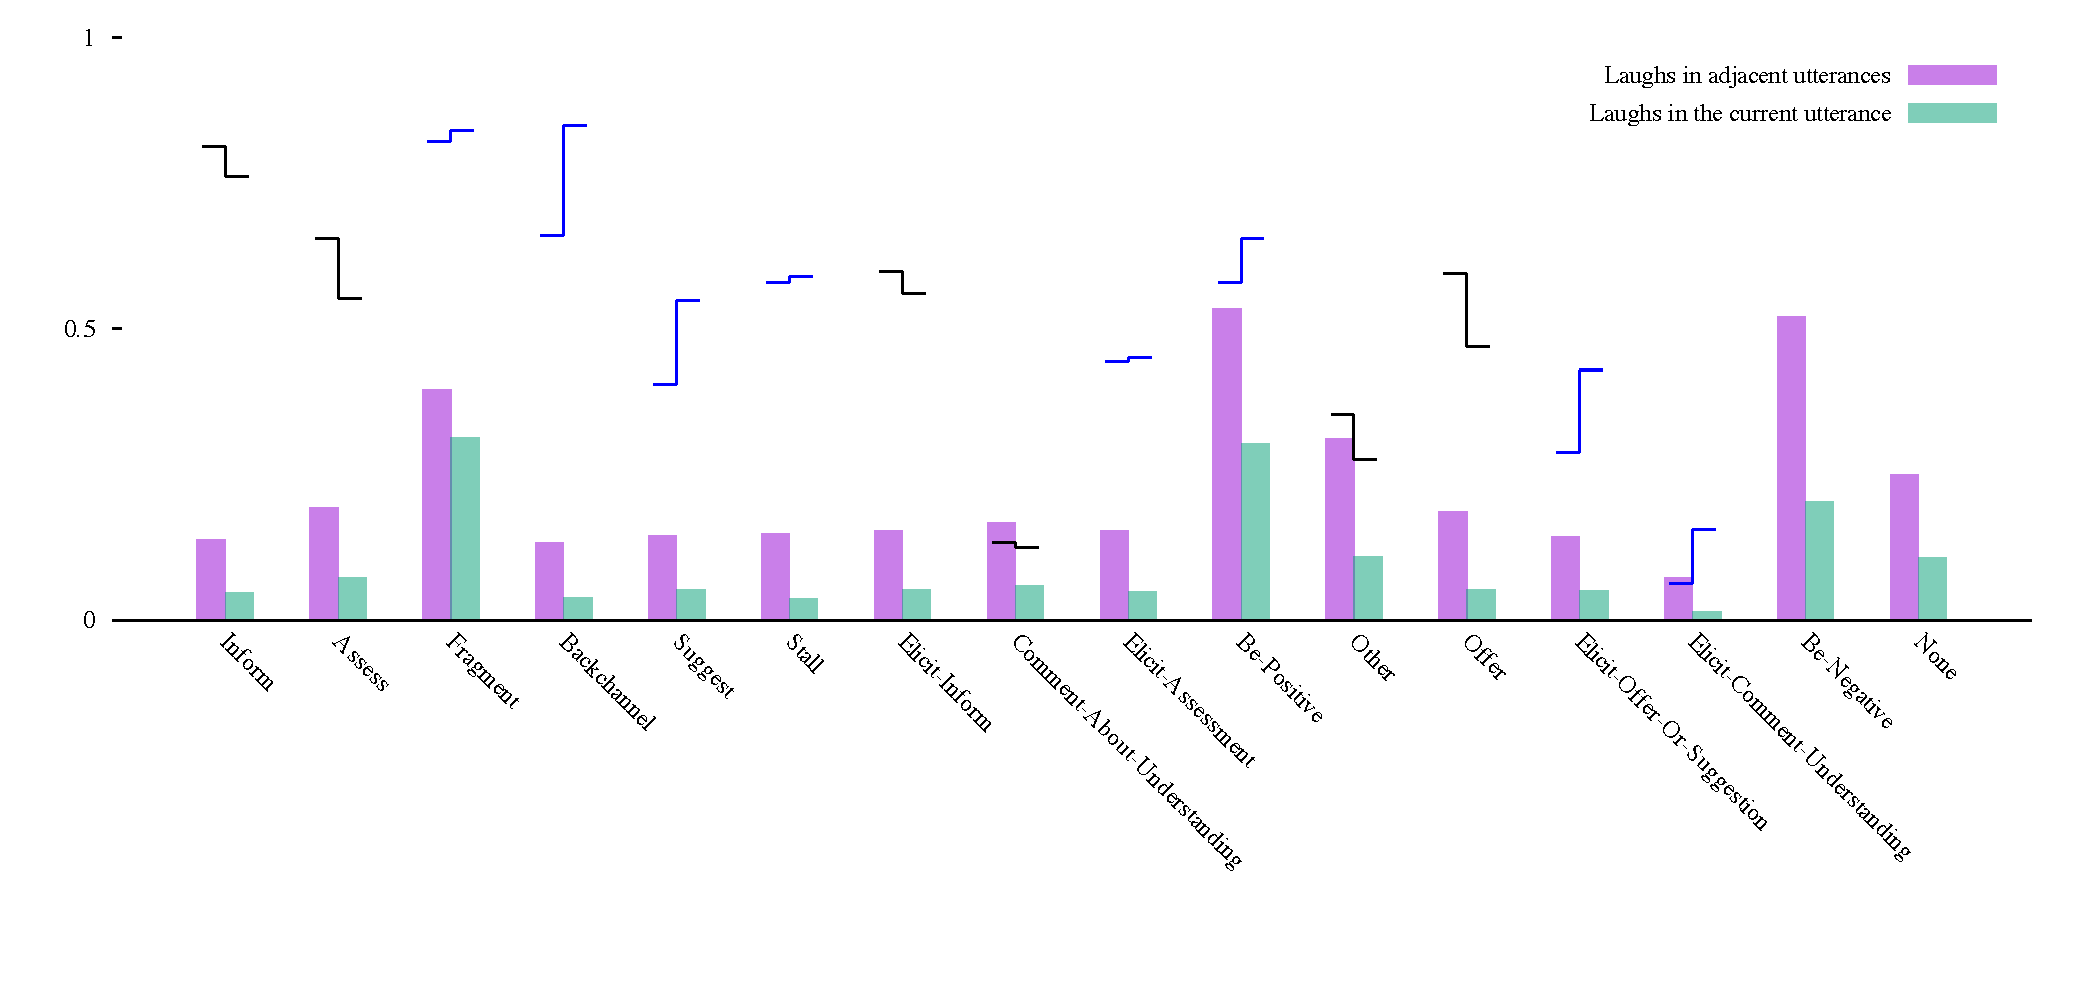
\includegraphics[width=\textwidth]{img/AMI-DA-bertLvsNL.pdf}
  \caption{Change in accuracy for each AMI dialogue act. Positive changes when adding laughter are shown in blue. Vertical bars indicate how often dialogue act is associated with laughter.}
\end{figure*}
% TODO per dialogue act analysis
% DONE compare impacts of CNN vs BERT
% DONE for both AMI and SWDA
% ? 

\subsection{Experiment 2: Impact of pre-training vs. fine-tuning} \label{sec:experiment2} % Bill
% - compare i) pre-trained BERT with freezing ii) pretrained with no freezing iii) randolmly initialized
Next, we take a direct look at how pre-training affects BERT's performance as an utterance encoder for our DAR model.
In particular, we consider the performance of DAR models with three different utterance encoders:
\begin{itemize}
  \item \texttt{BERT} -- pre-trained BERT without fine-tuning 
  \item \texttt{BERT-FT} -- pre-trained BERT with DAR fine-tuninig 
  \item \texttt{BERT-RI} -- randomly initialized BERT with dAR fine-tuning 
\end{itemize}

\begin{table}[]
\centering 
\begin{tabular}{@{}lll@{}}
\toprule
                 & SWDA  & AMI-DA \\ \midrule
\texttt{BERT}       & 55.61 & 46.59  \\
\texttt{BERT-FT}    & 76.93 & 66.94  \\
\texttt{BERT-RI}    & 73.80 & 61.53  
\end{tabular}
  \caption{Micro-average DAR recall}
  \label{table:exp2-avg}
\end{table}    

The pre-trained model performs better than the randomly initialized model by several percentage points on both DA corpora (table \ref{table:exp2-avg}). 
These results suggest that BERT's extensive pre-training do provide some useful information for dialogue act recoginition.
However, we note that pre-training is not enough: the poor performance of the frozen \texttt{BERT} model indicates that fine-tuning is important for BERT's performance as an utterance encoder.
These observations raise two questions.
First, how does BERT's pre-training help with DAR? 
And second, in what way are the representations learned by pre-trained BERT lacking?
In other words, what is the contribution of fine-tuning?

To help answer these questions, we compare performance of the above three models by dialogue act tag.

% TODO: add per dialogue act accuracy figures

\paragraph{Fine-tuning and laughter}
Since the laughter token doesn't appear in the original BERT vocabulary, only fine-tuned models can meaningfully make use of laughter in utterance representations. 
This gives us another opportunity to assess whether laughter is useful in dialogue act recognition.
We find that although \%4.6 of utterances in SWDA contain laughter, \%7.3 of utterances misclassified by \texttt{BERT} but correctly classified by \texttt{BERT-FT} contain laughter, suggesting that the fine-tuned encoder makes use of laughter. 
For AMI-DA, the effect is less pronounced, but still present§: \%8.5 of utterances contain laughter, and \%9.6 of utterances where fine-tuning makes a difference contain laughter.

\subsection{Experiment 3: Impact of in-domain pre-training} \label{sec:experiment3} % Bill
% - pre-train AMI+SWBD -> train SWDA/AMI-DA -> test SWDA/AMI-DA
% - pre-traing tasks: 1) next utterance, 2) masked token, 3) both ?
% - compare frozen with no dialogue pre-training vs pre-trained on dialogue w.r.t. L/NL (same as in Experiment 1)

Next, we assess the effect of in-domain pre-training of BERT's performance as an utterance encoder.\footnote{
In-domain pre-training is sometimes referred to as fine-tuning, but we reserve that term for task-specific training on labeled data.}
We construct pre-training corpora from the SWDA portion of the un-labelled Switchboard corpus and from the entire AMI corpus (including meetings with no human-annotated DA tags that are not included in the DAR training set).
In both cases, we exclude dialogues that are reserved for DAR testing.

We use the same pre-training task described by \citet{devlinBERTPretrainingDeep2018}, which combines masked token prediction and next sentence (utterance) detection. 
Distractor utterances are drawn at random from another dialogue in the corpus
and each epoch is generated separately so that different distractor sentences appear each time.
We then performed DAR fine-tuning and inference with the in-domain pre-trained BERT models just as before.

For AMI, in-domain pre-training offers a modest performance boost, but there is no discernable effect in the case of Switchboard.
Indeed, when BERT is frozen during fine-tuning, the model that received no additional pre-training performs better by more than 3 percentage points (table \ref{tab:exp3-recall}).

\begin{table}[]
\begin{tabular}{@{}lll@{}}
\toprule
                       & SWDA  & AMI-DA \\ \midrule
in-domain pre-training & 77.02 & 68.64  \\
no fine-tuning         & 52.30 & 48.05  \\ \midrule
standard pre-training  & 76.93 & 66.94  \\
no fine-tuniing        & 55.61 & 46.59  \\ \bottomrule
\end{tabular}
  \caption{Micro-average DAR recall for different pre-training schemas.}
  \label{tab:exp3-recall}
\end{table}

We found no discernable difference between pre-traininig on dialogues from the same corpus and pre-traininig on the combined corpus.
These results could be explained by the relatively small size of the dialogue corpora.

%\subsection{Experiment 4: Cross-domain pre-training (if time permits)} \label{sec:experiment4} % Bill
%  - cross-domain pre-training
\section{Related work} % add references first
Dialogue act recoginition
\begin{itemize}
  \item \citet{pragstVectorRepresentationUtterances2018} -- dialogue vector models. Uses vector-manual DA tag correspondance to argue for semantic relevance of their vector models (related to how we use DA tagging to verrify BERT usefulness)
  \item \citet{cerisaraEffectsUsingWord2vec2017} -- standard pre-trained word embeddings do not help for DAR in any of three tested languages (English, French, Czech)
  \item \citet{kalchbrennerRecurrentConvolutionalNeural2013} -- DAR model similar to our architecture. Uses an RNN ``discourse model'' and a CNN similar to our baseline encoder
  \item \citet{khanpourDialogueActClassification2016} -- Deep LSTM utt representation. No notion of context. Finds word vectors are useful.
  \item \citet{tranPreservingDistributionalInformation2017} -- Sequential DA prediction with uncertainty propegation
  \item \citet{chenDialogueActRecognition2017} -- SOTA? SWDA DAR using attention and CRF over utterances
  \item \citet{ortegaNeuralbasedContextRepresentation2017} -- SWDA DAR with attention-based context representations and CNN utterance representations
  \item \citet{shenNeuralAttentionModels2016} -- Uses attention for utt encoding in DAR. No notion of context, I think.
  \item \citet{tranHierarchicalNeuralModel2017} -- RNNs at both the utteranec and dialogue level. Also attention. Very similar to our architecture.
\end{itemize}

Pre-training/transfer learning for dialogue
\begin{itemize}
  \item \citet{mehriStructuredFusionNetworks2019} -- ``Structured fusion networks''. Traditional dialogue system design with neural models.
  \item \citet{chenSemanticallyConditionedDialog2019a} -- uses BERT for response generation
  \item \citet{baoPLATOPretrainedDialogue2019} -- pre-traininig for dialogue generation
  \item \citet{mehriPretrainingMethodsDialog2019} -- looks at various dialogue tasks using pre-training, including DAR and using BERT
  \item \citet{vigComparisonTransferLearningApproaches} -- Transfer learning for response selection
\end{itemize}


\section{Discussion} % add items to discuss
\begin{itemize}
  \item RoBERTa training scheme finds that next sentence prediction is of little importance. Is this true for us too? (suspect not due to discourse importance). see: https://github.com/huggingface/transformers/issues/1622
  \item Issues related to working with transcribed speech: Different kinds of laughter are all represented by the same token. Does transcription orthography capture prosidy? We know prosidy is useful for DAR (Jurafsky).
\end{itemize}

\bibliography{acl2020}
\bibliographystyle{acl_natbib}

\end{document}
